% Auto-generated by experiments/plot_scaled_derivative_families.py.
% Requires \usepackage{pgfplots} and \pgfplotsset{compat=1.18}.
% Figure label suggestion: \label{fig:scaled-exit-hgp}
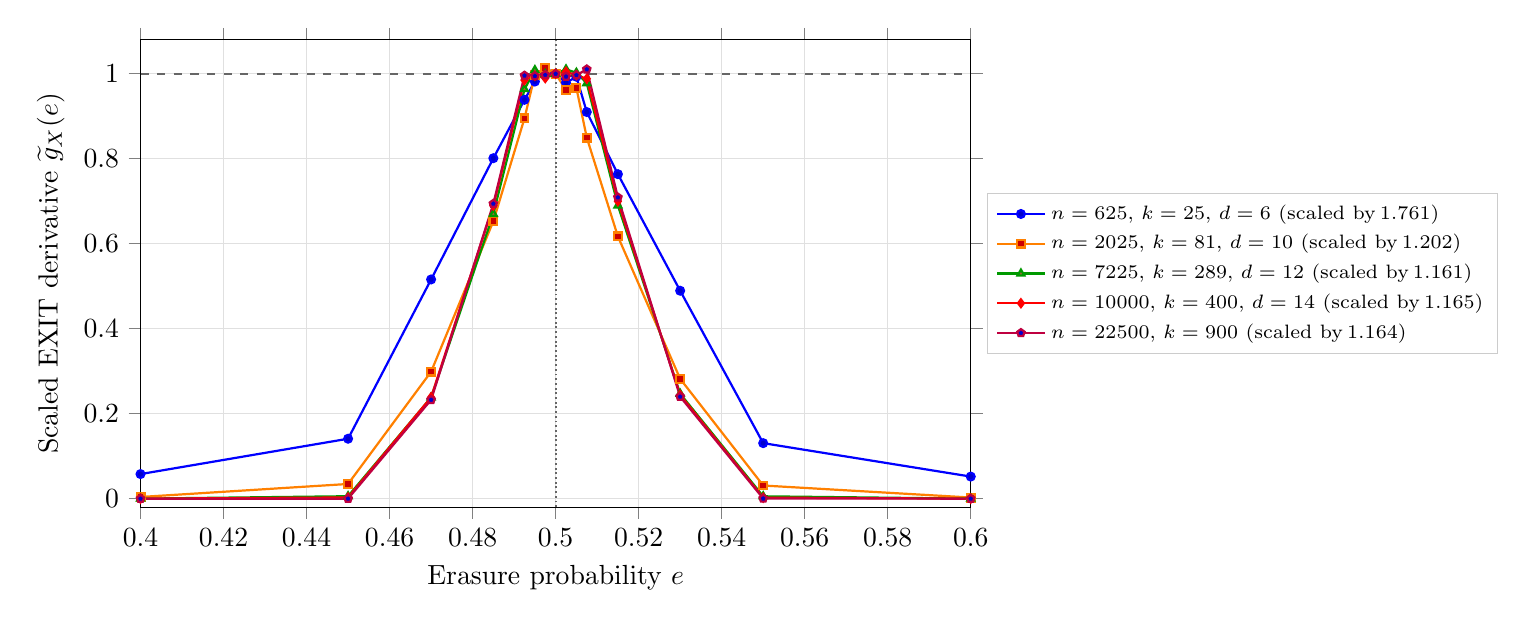
\begin{tikzpicture}
\begin{axis}[
  name=scaledEXITHGPAxis,
  width=\linewidth,
  height=0.62\linewidth,
  xlabel={Erasure probability $e$},
  ylabel={Scaled EXIT derivative $\widetilde g_X(e)$},
  xmin=0.4, xmax=0.6,
  ymin=-0.02, ymax=1.08,
  grid=both,
  major grid style={black!12},
  minor grid style={black!6},
  tick align=outside,
  legend cell align={left},
  legend style={draw=black!20, fill=white, at={(1.02,0.5)}, anchor=west, font=\scriptsize},
]
\addplot[black!60, densely dotted, line width=0.7pt, forget plot] coordinates {(0.5,-0.02) (0.5,1.08)};
\addplot[black!60, dashed, line width=0.7pt, forget plot] coordinates {(0.4,1) (0.6,1)};
\addplot+[color=blue, mark=*, mark size=1.4pt, line width=0.8pt]
coordinates {(0.4,0.0578873239437) (0.45,0.141046277666) (0.47,0.515895372233) (0.485,0.801251956182) (0.4925,0.938732394366) (0.495,0.981690140845) (0.4975,1.00985915493) (0.5,1) (0.5025,0.978873239437) (0.505,0.992957746479) (0.5075,0.90985915493) (0.515,0.763693270736) (0.53,0.489336016097) (0.55,0.130684104628) (0.6,0.0519718309859)};
\addlegendentry{$n=625$, $k=25$, $d=6$ ($\mathrm{scaled\ by}\,1.761$)}
\addplot+[color=orange, mark=square*, mark size=1.4pt, line width=0.8pt]
coordinates {(0.4,0.00397862232779) (0.45,0.0346114692908) (0.47,0.298778418731) (0.485,0.653074689892) (0.4925,0.895190023753) (0.495,0.99703087886) (0.4975,1.01365795724) (0.5,1) (0.5025,0.961995249406) (0.505,0.96674584323) (0.5075,0.849762470309) (0.515,0.617049353391) (0.53,0.281981676281) (0.55,0.0309636918901) (0.6,0.00267220902613)};
\addlegendentry{$n=2025$, $k=81$, $d=10$ ($\mathrm{scaled\ by}\,1.202$)}
\addplot+[color=green!60!black, mark=triangle*, mark size=1.4pt, line width=0.8pt]
coordinates {(0.4,9.64320154291e-05) (0.45,0.00577444092391) (0.47,0.238095238095) (0.485,0.669988213865) (0.4925,0.963677274188) (0.495,1.00851816136) (0.4975,0.999035679846) (0.5,1) (0.5025,1.01028608165) (0.505,1.00241080039) (0.5075,0.977659916426) (0.515,0.689881781492) (0.53,0.246980759517) (0.55,0.00556780089085) (0.6,6.42880102861e-05)};
\addlegendentry{$n=7225$, $k=289$, $d=12$ ($\mathrm{scaled\ by}\,1.161$)}
\addplot+[color=red, mark=diamond*, mark size=1.4pt, line width=0.8pt]
coordinates {(0.4,2.3301875801e-05) (0.45,0.00285447978562) (0.47,0.238561275611) (0.485,0.689813196629) (0.4925,0.985203308866) (0.495,0.99533962484) (0.4975,0.989863684027) (0.5,1) (0.5025,1.00489339392) (0.505,0.996737737388) (0.5075,0.98829080741) (0.515,0.700040131008) (0.53,0.244087149015) (0.55,0.00245501905761) (0.6,2.3301875801e-05)};
\addlegendentry{$n=10000$, $k=400$, $d=14$ ($\mathrm{scaled\ by}\,1.165$)}
\addplot+[color=purple, mark=pentagon*, mark size=1.4pt, line width=0.8pt]
coordinates {(0.4,0) (0.45,2.95617470993e-05) (0.47,0.232687901855) (0.485,0.694131172041) (0.4925,0.995732022763) (0.495,0.994568028971) (0.4975,0.997206414899) (0.5,1) (0.5025,0.993429901707) (0.505,0.996896016555) (0.5075,1.01042421107) (0.515,0.708926826464) (0.53,0.240026605572) (0.55,0.000450816643264) (0.6,0)};
\addlegendentry{$n=22500$, $k=900$ ($\mathrm{scaled\ by}\,1.164$)}
\end{axis}
\end{tikzpicture}
